\documentclass[xcolor=dvipsnames,table]{beamer}

\usepackage{latexsym}
\usepackage[utf8]{inputenc}
\usepackage[brazil]{babel}
\usepackage{amssymb}
\usepackage{amsmath}
\usepackage{stmaryrd}
\usepackage{fancybox}
\usepackage{datetime}
\usepackage[T1]{fontenc}
\usepackage{graphicx}
\usepackage{graphics}
\usepackage{url}
\usepackage{algorithmic}
\usepackage{algorithm}
\usepackage{acronym}
\usepackage{array}
\usepackage[normalem]{ulem}

\newtheorem{definicao}{Definio}
\newcommand{\tab}{\hspace*{2em}}

\mode<presentation>
{
  \definecolor{colortexto}{RGB}{0,0,0}
 
  \setbeamertemplate{background canvas}[vertical shading][ bottom=white!10,top=white!10]
  \setbeamercolor{normal text}{fg=colortexto} 

  \usetheme{Warsaw}
}

\title{Decidibilidade} 

\author{
  Esdras Lins Bispo Jr. \\ \url{bispojr@ufg.br}
  } 
 \institute{
  Teoria da Computação \\Bacharelado em Ciência da Computação}
\date{\textbf{07 de junho de 2016} }

\logo{
\includegraphics[width=1cm]{images/ufgJataiLogo.png}}

\begin{document}

	\begin{frame}
		\titlepage
	\end{frame}

	\AtBeginSection{
		\begin{frame}{Sumário}%[allowframebreaks]{Sumário}
    		\tableofcontents[currentsection]
    		%\tableofcontents[currentsection, hideothersubsections]
		\end{frame}
	}

	\begin{frame}{Plano de Aula}
		\tableofcontents
		%\tableofcontents[hideallsubsections]
	\end{frame}
	
	\begin{frame}{Bônus (0,5 pt)}
		\begin{block}{Desafio}
			\begin{itemize}
				\item {\bf Problema 4.12:} \\Seja $A = \{ \langle R, S \rangle$ | $R$ e $S$ são expressões regulares e L($R$) $\subseteq$ L($S$)$\}$. Mostre que $A$ é decidível.
                \item Candidaturas até amanhã (07 de junho, 09h30); 
                \item Apresentação e resposta por escrito $\rightarrow$ \\Segunda (14 de junho, 11h30); 
                \item 20 minutos de apresentação.
			\end{itemize}
		\end{block} 
        \begin{block}{Candidato}
        	???
        \end{block}
	\end{frame}
    
    \section{Pensamento}
	\begin{frame}{Pensamento}
  		\begin{center}
    		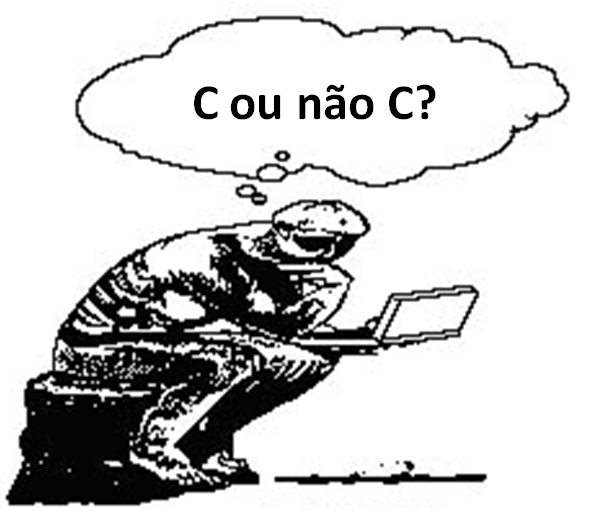
\includegraphics[width=7cm]{images/pensamento.png}
  		\end{center}
	\end{frame}
	
	\begin{frame}{Pensamento}
		\begin{columns}
			\column{.4\textwidth}  		
		  		\begin{center}
		    		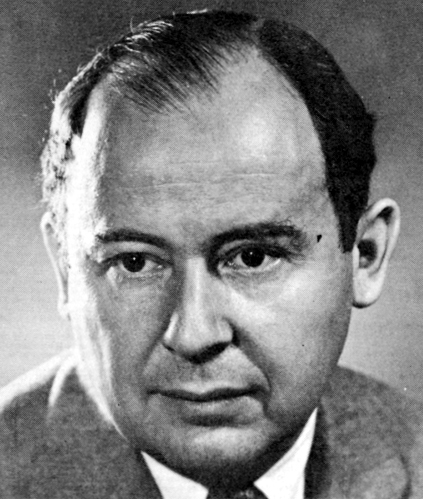
\includegraphics[height=.6\textheight]{images/vonNeumann.jpg}
		  		\end{center}
			\column{.6\textwidth}  		
				\begin{block}{Frase}
					\begin{center}
						{\large Any one who considers arithmetical methods of producing random digits is, of course, in a state of sin.}
					\end{center}
				\end{block}		  		
		  		\begin{block}{Quem?}
		  			\begin{center}
						{\bf John von Neumann (1903-1957)} \\ Cientista da computação húngaro/americano.
					\end{center}
				\end{block}
		\end{columns}
	\end{frame}
	
%------------------------------------------

\section{Revisão}
	\subsection{Decidibilidade}
	\begin{frame}{Introdução}
		\begin{block}{Propósitos da Teoria da Computação}
			\begin{itemize}
				\item Conhecer o poder dos algoritmos;
				\item Explorar os limites da solubilidade algorítmica;
				\item Identificar algoritmos insolúveis.
			\end{itemize}
		\end{block}  
		\begin{block}{Por que devemos estudar insolubilidade?}
			\begin{itemize}
				\item Relaxamento dos requisitos;
				\item Conhecimento das limitações dos modelos computacionais.
			\end{itemize}
		\end{block}
	\end{frame}
	
	\begin{frame}{Linguagens Decidíveis}
		\begin{block}{Exemplos de Linguagens Decidíveis}
			São úteis porque
			\begin{itemize}
				\item Algumas linguagens decidíveis estão associadas a aplicações;
				\item Algumas linguagens aparentemente triviais não são decidíveis.
			\end{itemize}
		\end{block}
		\begin{block}{Problema da aceitação}
			Dado um modelo computacional $MC$ e uma cadeia de entrada $\omega$, identificar se $MC$ aceita $\omega$.
		\end{block}	
	\end{frame}
	
	\begin{frame}{Problema da aceitação para AFDs}
		\begin{block}{Problema da aceitação para AFDs}
			Dado um AFD $B$ e uma cadeia de entrada $\omega$, identificar se $B$ aceita $\omega$.
		\end{block}	
		\begin{block}{Problema}
			$A_{AFD} = \{ \langle B, \omega \rangle \mbox{ | } B \mbox{ é um AFD que aceita a cadeia de entrada } \omega \}$
		\end{block} 
		\begin{block}{Estratégia de Resolução}
			Resolver o problema da aceitação para AFDs é decidir se $\omega \in A_{AFD}$.
		\end{block}
	\end{frame}
	
	\begin{frame}{Problema da aceitação para AFDs}
		\begin{block}{Teorema 4.1}
			$A_{AFD}$ é uma linguagem decidível.
		\end{block} 
		\begin{block}{Ideia da Prova}
			$M$ = ``Sobre a entrada $\langle B, \omega \rangle$, em que $B$ é um AFD, e $\omega$, uma cadeia:
			\begin{enumerate}
				\item Simule $B$ sobre a entrada $\omega$;
				\item Se a simulação termina em um estado de aceitação, {\bf aceite}. Senão, {\bf rejeite}.''
			\end{enumerate}
		\end{block}
	\end{frame}
	
	\begin{frame}{Problema da aceitação para AFDs}
		\begin{block}{Detalhes de implementação}
			\begin{itemize}
				\item A entrada $\langle B, \omega \rangle$ representa um AFD e uma cadeia;
				\begin{itemize}
					\item Uma representação razoável de $B$ seria uma lista de seus cinco componentes: $Q, \Sigma, \delta, q_0$ e $F$;
					\item $M$ simula $B$ de forma que $M$ {\bf aceita} se $B$ estiver em um estado final, e {\bf rejeita}, caso contrário.
				\end{itemize}
			\end{itemize}
		\end{block}
	\end{frame}
	
	\begin{frame}{Problema da aceitação para AFNs}
		\begin{block}{Problema da aceitação para AFNs}
			Dado um AFN $B$ e uma cadeia de entrada $\omega$, identificar se $B$ aceita $\omega$.
		\end{block}	
		\begin{block}{Problema}
			$A_{AFN} = \{ \langle B, \omega \rangle \mbox{ | } B \mbox{ é um AFN que aceita a cadeia de entrada } \omega \}$
		\end{block} 
		\begin{block}{Estratégia de Resolução}
			Decidir se $\langle B, \omega \rangle \in A_{AFN}$.
		\end{block}
	\end{frame}	
	
	\begin{frame}{Problema da aceitação para AFNs}
		\begin{block}{Teorema 4.2}
			$A_{AFN}$ é uma linguagem decidível.
		\end{block} 
		\begin{block}{Prova}
			$N$ = ``Sobre a entrada $\langle B, \omega \rangle$, em que $B$ é um AFN, e $\omega$, uma cadeia:
			\begin{enumerate}
				\item Converta AFN $B$ para um AFD equivalente $C$, usando o procedimento para essa conversão dado no Teorema 1.39;
				\item Rode a MT $M$ do Teorema 4.1 sobre a cadeia $\langle C, \omega \rangle$;
				\item Se $M$ aceita, {\bf aceite}. Caso contrário, {\bf rejeite}.''
			\end{enumerate}
		\end{block}
	\end{frame}
	
	\begin{frame}{Problema da Vacuidade de uma Linguagem}
		\begin{block}{Descrição}
			Dada uma linguagem $L$, identificar se $L = \emptyset$.
		\end{block}	
		\begin{block}{Problema aplicado a AFDs}
			$V_{AFD} = \{ \langle A \rangle \mbox{ | } A \mbox{ é um AFD e } L(A) = \emptyset \}$
		\end{block} 
		\begin{block}{Estratégia de Resolução}
			Decidir se $\langle A \rangle \in V_{AFD}$.
		\end{block}
	\end{frame}	
	
	\begin{frame}{Problema da Vacuidade de uma Linguagem}
		\begin{block}{Teorema 4.4}
			$V_{AFD}$ é uma linguagem decidível.
		\end{block} \pause
		\begin{block}{Prova}
			A seguinte MT $T$ decide $V_{AFD}$.
			
			$T$ = ``Sobre a entrada $\langle A \rangle$, em que $A$ é uma AFD:
			\begin{enumerate}
				\item Marque o estado inicial de $A$;
				\item Repita até que nenhum estado novo venha a ser marcado;
					\begin{enumerate}
						\item Marque qualquer estado que tenha uma transição chegando nele a partir de qualquer estado que já está marcado.
					\end{enumerate}
				\item Se nenhum estado final estiver marcado, {\bf aceite}. Caso contrário, {\bf rejeite}.''
			\end{enumerate}
		\end{block}
	\end{frame}
	
	\section{Decidibilidade}
	
	\begin{frame}{Problema da Igualdade de Linguagens}
		\begin{block}{Descrição}
			Dadas duas linguagem $L_1$ e $L_2$, identificar se $L_1 = L_2$.
		\end{block}	\pause
		\begin{block}{Problema aplicado a AFDs}
			$EQ_{AFD} = \{ \langle A, B \rangle \mbox{ | } A$ e $B$ são AFDs e $L(A) = L(B) \}$
		\end{block} \pause
		\begin{block}{Estratégia de Resolução}
			Decidir se $\langle A, B \rangle \in EQ_{AFD}$.
		\end{block}
	\end{frame}		
	
	\begin{frame}{Problema da Igualdade de Linguagens}
		\begin{block}{Teorema 4.5}
			$EQ_{AFD}$ é uma linguagem decidível.
		\end{block} \pause
		\begin{block}{Lema 4.1}
			Iremos construir um AFD $C$ a partir de $A$ e $B$ de forma que $C$ aceita as cadeias que são aceitas por $A$ ou por $B$, mas não por ambas. Consequentemente, se $A$ e $B$ reconhecem a mesma linguagem, $C$ não aceitará nada. A linguagem de $C$ é
			\begin{center}
				$L(C) = \left( L(A) \cap \overline{L(B)} \right) \cup \left( \overline{L(A)} \cap L(B) \right)$
			\end{center}
		\end{block} \pause
		\begin{block}{Corolário}
			$L(C) = \emptyset$ \ $\leftrightarrow$ \ $L(A) = L(B)$
		\end{block}
	\end{frame}
	
	\begin{frame}{Problema da Igualdade de Linguagens}
		\begin{center}
    		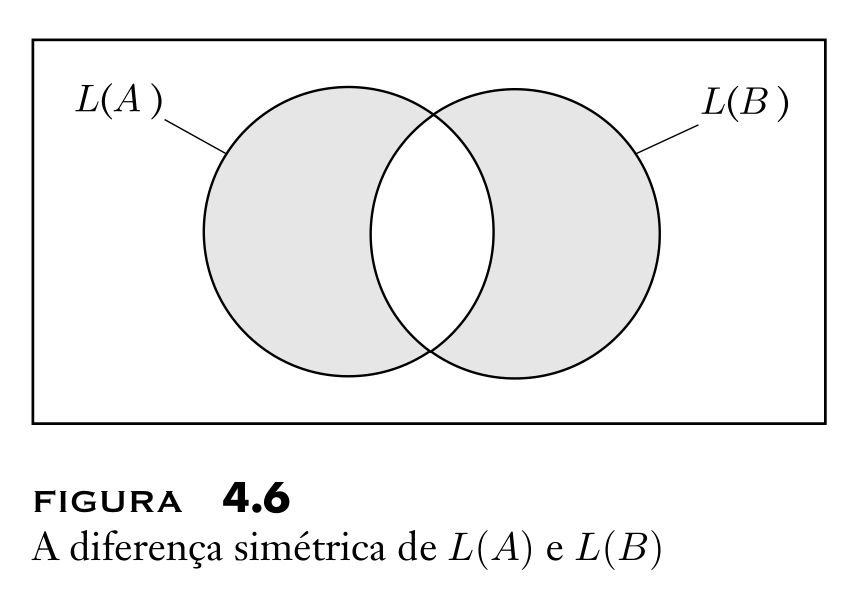
\includegraphics[width=9cm]{images/fig46.png}
  		\end{center}
	\end{frame}
	
	\begin{frame}{Problema da Igualdade de Linguagens}
		\begin{block}{Teorema 4.5}
			$EQ_{AFD}$ é uma linguagem decidível.
		\end{block} \pause
		\begin{block}{Prova}
			A seguinte MT $F$ decide $EQ_{AFD}$.
			
			$F$ = ``Sobre a entrada $\langle A, B \rangle$, em que $A$ e $B$ são AFDs:
			\begin{enumerate}
				\item Construa o AFD $C$ conforme descrito no Lema 4.1;
				\item Rode MT $T$ do Teorema 4.4 sobre a entrada $\langle C \rangle$;
				\item Se $T$ aceita, {\bf aceite}. Caso contrário, {\bf rejeite}.''
			\end{enumerate}
		\end{block}
	\end{frame}
	
	\begin{frame}{Teoremas sobre GLC}
		\begin{block}{Teorema 4.7}
			$A_{GLC}$ é uma linguagem decidível.
		\end{block}
		\begin{block}{Teorema 4.8}
			$V_{GLC}$ é uma linguagem decidível.
		\end{block}
		\begin{block}{Teorema 4.9}
			Toda LLC é decidível.
		\end{block} \pause
		\begin{alertblock}{Cuidado!}
			$EQ_{GLC}$ {\color{red} {\bf não}} é uma linguagem decidível.
		\end{alertblock}
	\end{frame}
	
	\begin{frame}{Relacionamento entre as classes de linguagens}
		\begin{center}
    		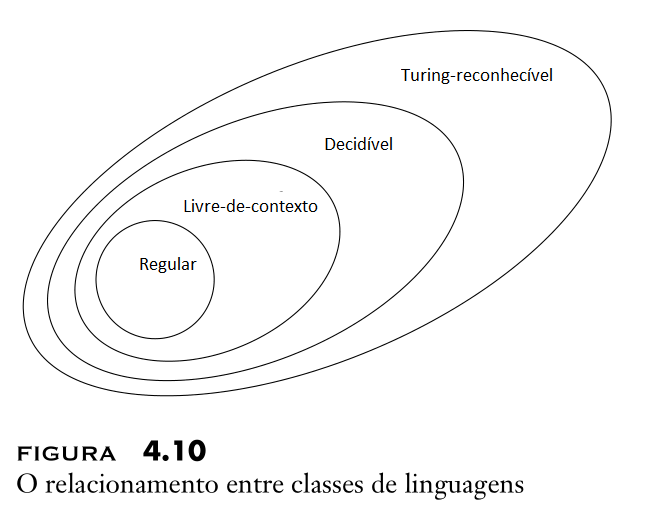
\includegraphics[width=9cm]{images/fig410.png}
  		\end{center}
	\end{frame}
	
	\subsection{O Problema da Parada}
	\begin{frame}{O Problema da Parada}
		\begin{block}{Problema da aceitação para MT}
			Dada uma MT $M$ e uma cadeia de entrada $\omega$, identificar se $M$ aceita $\omega$.
		\end{block}	\pause
		\begin{block}{Problema}
			$A_{MT} = \{ \langle M, \omega \rangle$  | $M$ é uma MT que aceita a cadeia de entrada $\omega \}$
		\end{block} \pause
		\begin{alertblock}{Teorema 4.11}
			$A_{MT}$ é indecidível.
		\end{alertblock}
	\end{frame}
	
	\begin{frame}{O Problema da Parada}
		\begin{block}{Considerações sobre o Teorema 4.11}
			$A_{MT}$ é Turing-reconhecível. Pois é possível construir $U$ da seguinte forma: \pause
			
			$U$ = ``Sobre a entrada $\langle M, \omega \rangle$, em que $M$ é uma MT e $\omega$ uma cadeia:
			\begin{enumerate}
				\item Simule $M$ sobre a entrada $\omega$;
				\item Se $M$ em algum momento entra no seu estado de aceitação, {\bf aceite}; se $M$ em algum momento entra em seu estado de rejeição, {\bf rejeite}.''
			\end{enumerate}
		\end{block}	\pause
		\begin{alertblock}{Problema da Parada}
			Não é possível construir uma MT que decida $A_{MT}$.
		\end{alertblock} 
	\end{frame}
	
	\begin{frame}{O Problema da Parada}
		\begin{block}{Máquina de Turing Universal}
			É uma MT capaz de simular qualquer outra MT. \\A MT $U$ apresentada anteriormente é uma MT Universal.
		\end{block} \pause
		\begin{exampleblock}{Contribuição importante}
			A MT Universal estimulou o desenvolvimento de computadores com programas armazenado.
		\end{exampleblock} 
	\end{frame}
	
	\begin{frame}{O Problema da Parada}
		\begin{center}
    		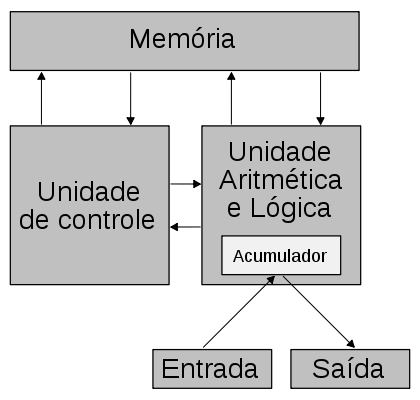
\includegraphics[width=6cm]{images/arqVonNeumann.png}
    		
    		{\bf Figura:} Arquitetura de von Neumann (1945).
  		\end{center}
	\end{frame}
	
	\begin{frame}{Método da diagonalização}
		\begin{columns}
			\column{.4\textwidth}  		
		  		\begin{center}
		    		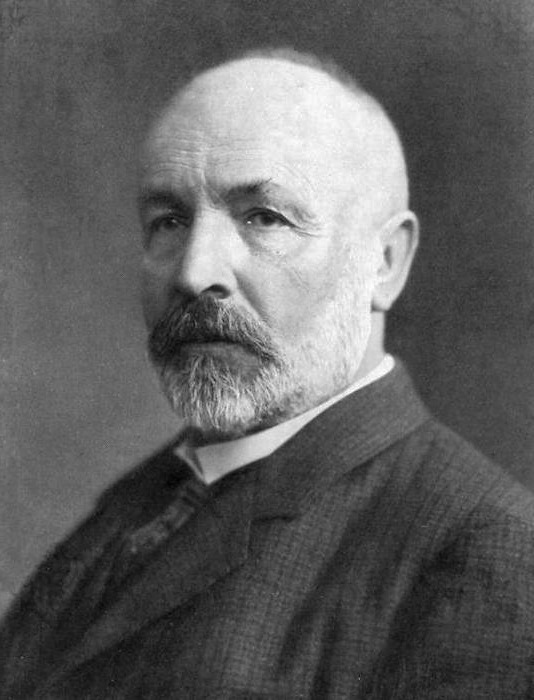
\includegraphics[height=.6\textheight]{images/cantor.jpg}
		  		\end{center}
			\column{.6\textwidth}  		
				\begin{block}{Contribuição}
					\begin{center}
						{\large Criou o método da diagonalização em 1873.}
					\end{center}
				\end{block}		  		
		  		\begin{block}{Quem?}
		  			\begin{center}
						{\bf George Cantor (1845-1918)} \\ Matemático russo.
					\end{center}
				\end{block}
		\end{columns}
	\end{frame}
	
	\begin{frame}{Método da diagonalização}
		\begin{alertblock}{Problema}
			Se temos dois conjuntos infinitos, como podemos dizer se um conjunto é maior que o outro (ou se eles têm o mesmo tamanho)?
		\end{alertblock} \pause
		\begin{block}{Conjuntos finitos}
			Podemos utilizar o método da contagem.
		\end{block} \pause
		\begin{exampleblock}{Proposta de Cantor}
			Dois conjuntos finitos têm o mesmo tamanho se os elementos de um deles puder ser emparelhados com os elementos do outro. Basta estendermos essa ideia para os conjuntos infinitos!
		\end{exampleblock}
	\end{frame}
	
	\begin{frame}{Método da diagonalização}
		\begin{block}{Função um-para-um}
			Sejam dois conjuntos $A$ e $B$ e uma função $f$ de $A$ para $B$. Dizemos que $f$ é {\bf um-para-um} se ela nunca mapeia dois elementos diferentes para um mesmo lugar (ou seja, $f(a) \not= f(b)$ sempre que $a \not= b$).
		\end{block}	\pause	
		\begin{block}{Função Sobrejetora}		
			Uma função $f$ é {\bf sobrejetora} se ela atinge todo elemento de $B$ \\(ou seja, se para todo $b \in B$ existir um $a \in A$ tal que $f(a) = b$).
		\end{block} 
	\end{frame}
	
	\begin{frame}{Método da diagonalização}
		\begin{block}{Correspondência}
			Uma {\bf correspondência} é uma função que é tanto um-para-um, quanto sobrejetora. Em uma correspondência $f : A \rightarrow B$, todo elemento de $A$ é mapeado para um único elemento de $B$ e cada elemento de $B$ tem um único elemento de $A$ mapeando para ele. 
		\end{block} \pause
		\begin{block}{Tamanho de conjuntos}
			Dois conjuntos $A$ e $B$ são de {\bf mesmo tamanho} se existe uma correspondência de $A$ para $B$.
		\end{block}
	\end{frame}
	
	\begin{frame}
		\titlepage
	\end{frame}
	
\end{document}